
\chapter{Standardizing and automating recommendation experiments}
\label{ch:librec-auto}

Recommender systems are complex. They integrate the individual needs of users with the characteristics of particular domains of application which may span items from large and potentially heterogeneous collections. Extensive experimentation is required to understand the multidimensional properties of recommendation algorithms and the fit between algorithm and application, particularly in understudied areas like fairness-aware recommendation. To address these issues we created \libauto{}, a tool that automates many aspects of off-line batch recommender system experimentation.  

It has a large library of state-of-the-art and historical recommendation algorithms and a wide variety of evaluation metrics. It further supports the study of diversity and fairness in recommendation through the integration of re-ranking algorithms and fairness-aware metrics. It supports declarative configuration for reproducible experiment management and supports multiple forms of hyperparameter optimization.

\todo[inline]{make sure the descriptions for the config file and the new config file match}

% In this chapter, we describe the enhancements we made to LibRec. These enhancements include metrics for various classes of fairness definitions, extension of the experimental model to support result re-ranking and a library of associated re-ranking algorithms, and additional support for experiment automation and reporting, capability of parallelization, optimization, and etc.

% \librecato{} was created for our internal research needs such as having standard fairness-aware algorithms or re-rankers and having standard metrics to assess different types of biases, automating and parallelizing experiments, and etc. Many of the extended features weren't available in the existing recommendation tools, especially the capability of running experiments on fairness and diversity in recommendation.

In this chapter, we provide detailed capabilities of \libauto{} in its current release, including the features of this system and how they embed recommender system experiments, the typical usage of the system, and description of plans for future releases.


\section{Introduction}
\label{sec:librec_intro}

\libauto{} is a Python-based tool for recommender systems experimentation\footnote{https://librec-auto.readthedocs.io/en/latest/quickstart.html}. It is designed to support researchers by automating experimental methodology, thereby making experimental results more reproducible, and allowing simplified access to the large collection of algorithm implementations found in the LibRec platform. The system supports off-line batch evaluation in which ratings data (either explicit or implicit) are divided into training and test sets and the algorithm is evaluated on test set performance. Although other evaluation methods are gaining currency, particularly those that support reinforcement learning \cite{joachims2018reveal,joachims2019reveal,joachims2020reveal}, this type of evaluation is still extremely common in research practice and in educational settings. 

% \textbf{Reproducibility in Recommender Systems Research}
Reproducibility is a challenge in recommender systems research~\cite{said2014comparative,beel2016towards,sun2020we}, particularly in the areas that are not well-established such as fairness-aware recommendation. Even minor differences in parameters and experimental settings can yield incompatible results, which make it difficult to provide definitive answers about the relative properties of different algorithms \cite{Said2015Replicable}. Additionally, many of the existing libraries are not comprehensive. They mostly support experimentation for a very specific class of algorithms to demonstrate a specific set of results, making it difficult to readily re-use their capabilities for general research purposes. 

We believe that progress towards reproducibility is best supported by providing a platform on which comparative experiments can be conducted using declarative experimental configuration (so that experimental settings can be easily shared), with pre-implemented methodological workflows, and with a large library of algorithms for easy of benchmarking against prior work. \libauto{} is such a platform and it has been steadily enhanced over multiple years to meet the needs of researchers.


\section{LibRec and librec-auto}
\label{sec:libauto}

\libauto{} was originally designed as an open-source command-line Python package providing a wrapper for the LibRec recommender systems algorithm library\footnote{https://guoguibing.github.io/librec/index.html}. LibRec is a Java-based recommendation generation platform, available under the GPL 3.0 open-source license. It was introduced in 2015 \cite{guo2015librec}, and is maintained by a group led by Professor Guibing Guo at Northeastern University, Shenyang, China. Their group has implemented a large library of recommendation algorithms (more than 70 as of this writing) drawn from the recommender systems research literature. In addition to numerous algorithms, the LibRec platform supports a variety of evaluation metrics and evaluation methodologies.

Despite the significant capabilities of LibRec, we found that for practical experimentation and reproducibility research, the system by itself is not sufficient. For example, intermediate computational outputs, such as recommendation results, cannot be reused as input for new evaluation metrics. If an experimenter runs an experiment and then wishes to follow-up and explore additional properties of the results, LibRec would require re-execution of the entire set of recommendation computations. In addition, result re-ranking is not supported because of the close tie between algorithm execution and result evaluation built into LibRec. This makes it difficult to use LibRec as it is to explore the areas of fairness-aware and diversity-enhanced recommendation.

\libauto{} was conceived and implemented as a wrapper for core aspects of LibRec's functionality, in particular, to control and organize inputs (experiment configurations) and outputs (predictions and metric calculations), while preserving an experimenter's ability to access the large collection of implemented algorithms and metrics found in LibRec. Based on our internal research needs, we have extended this platform in a number of ways, particularly to support research in fairness-aware recommendation. We have also enhanced LibRec with a suite of metrics for measuring the fairness of recommendation outcomes. In addition, the tool now supports recommendation re-ranking, a common approach to enhancing fairness, diversity, and other non-accuracy properties of recommendation outcomes.

Except for a small chunk of Java wrapper code, \libauto{} is implemented in Python and (because it inherits heavily from LibRec) is available under the same GPL 3.0 license. It can be installed using the \texttt{pip} package manager or by downloading the source package from GitHub\footnote{https://github.com/that-recsys-lab/librec-auto}. Because of its ease of configuration and use, \libauto{} also supports students and teachers in learning about recommendation algorithms and their evaluation. The system has been used for courses at the Technical University of Eindhoven and the University of Colorado, Boulder. 

\section{Key Features}
\label{sec:libauto_keyfeatures}

A sketch of the functionality of \libauto{} is provided in Figure~\ref{fig:librec-auto}. As the figure indicates, LibRec is encapsulated by \libauto{}, and its various component elements are used to execute particular portions of the experimental workflow. The user experience of the system is organized around the concept of a \textit{study}, which involves experimentation with a single data set and a single recommendation algorithm. Multiple hyperparameters may be investigated as part of a study, either through grid search or black-box optimization as described in Section \ref{subsec:libauto_opt}. Each combination of hyperparameters is evaluated through an \textit{experiment}, which may entail multiple training / test iterations if cross-validation is used. Although the figure indicates a straight-line of execution, parallelism is built into \libauto{} at the level of experiment execution. Because experiments can have lengthy execution times, the post-processing phase allows for integration with messaging platforms, including Slack, so that experimenters are notified when their tasks are complete. These messages can include visualizations of experimental output, to provide a quick overview of results.

\begin{figure*}[!htb]
    \centering
    % 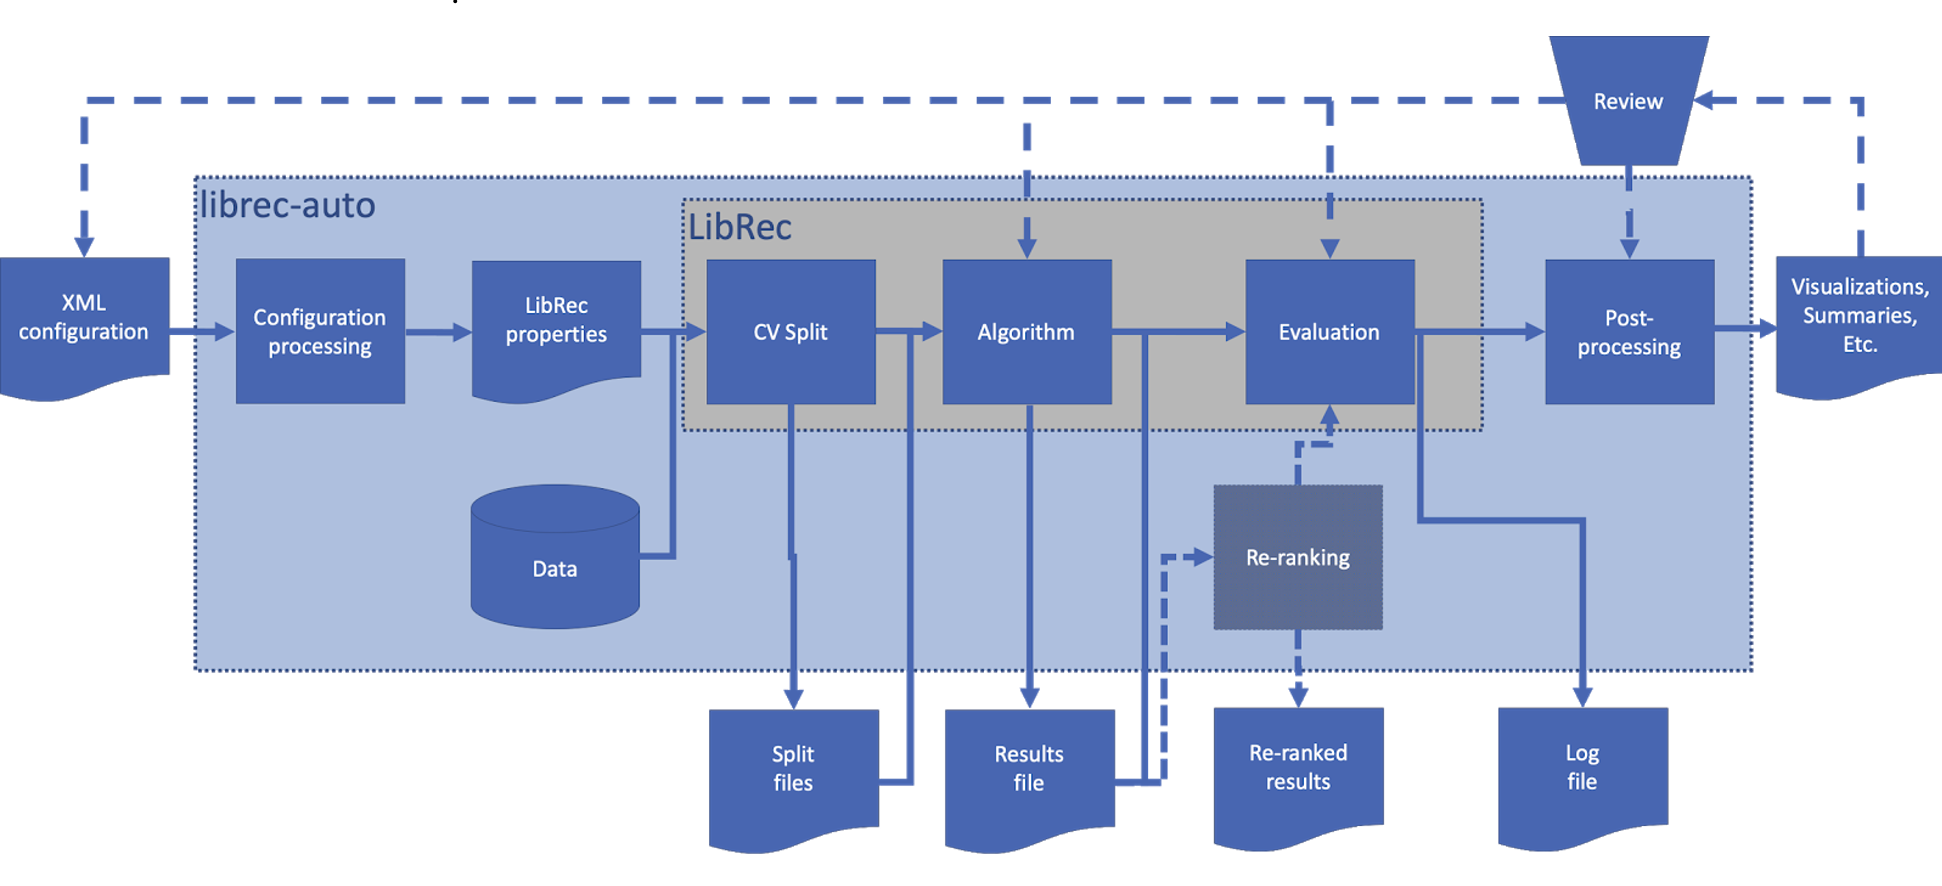
\includegraphics[width=5.25in]{imgs/la/librec-auto-diagram2.png}
    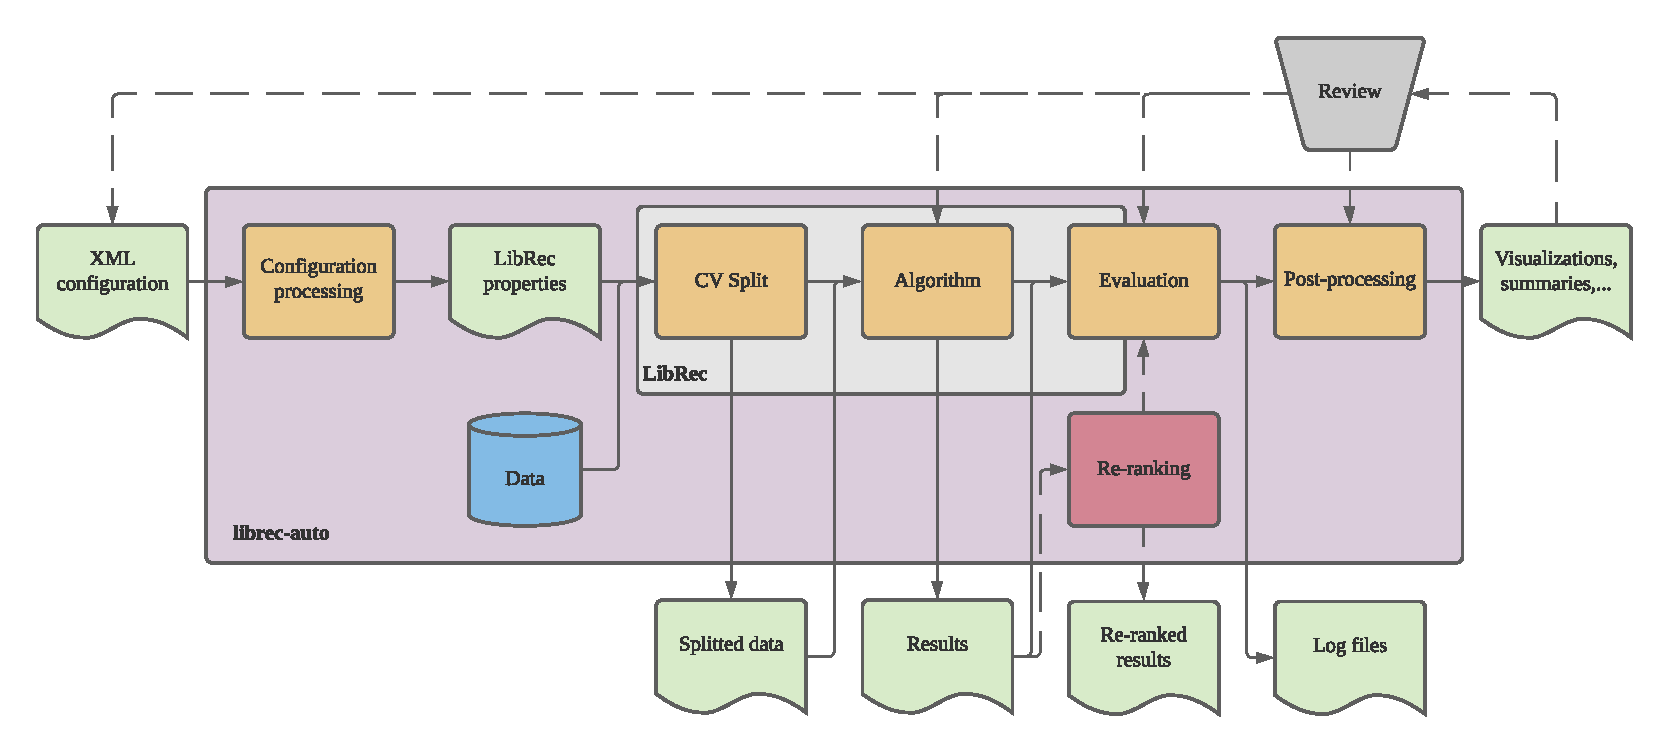
\includegraphics[width=0.95\linewidth]{imgs/la/workflow.pdf}
    \caption{Schematic of experimentation workflow with \libauto{}. The LibRec library (Java, shown in grey) is encapsulated by \libauto{} (Python, shown in purple), which manages configuration, experimental outputs and post-processing. Added from \cite{mansoury2018automating} is the new re-ranking module shown in red.}
    \label{fig:librec-auto}
    \vspace{-0.15in}
\end{figure*}

We can follow the workflow of a study through the processes depicted in Figure \ref{fig:librec-auto}.

\begin{description}

    \item [XML configuration] The experimenter designs a study and crafts a configuration file. The current release of \libauto{} includes a simple set-up wizard to automate some aspects of this process.

    \item [Configuration processing] The system processes the configuration file and produces internal data sources necessary for the study. These include folders for the experiments to be run, experiment-specific configuration files, and a translation of the LibRec-specific parts of the configuration into the key-value properties file that LibRec consumes.

    \item [CV split] The ratings data file is processed, and cross-validation train / test splits are produced. Ratings data is assumed to be in the form of a CSV file of sparse $\langle user, item, rating \rangle$ triples. Unlike vanilla LibRec, split files are saved, so that they can be used for further analysis, calculation of training data properties, for example, or for use by non-LibRec recommendation libraries.

    \item [Algorithm] The configured recommendation generation algorithm from LibRec is run, producing predictions over the training data. Depending on the nature of the evaluation metric, it will either generate a prediction for each training data triple or it will generate a ranked list of recommendations for each user in the training data. 
    
    \item [Re-ranking] (optional) If the study uses a re-ranking algorithm, the output of the (list-generating) recommender is input to this algorithm, and a new list of re-ranked results is produced for each user. The system includes a set of re-ranker implementations (see below), written as Python scripts. 

    \item [Evaluation] The metrics established in the configuration file are executed over the recommendation results. As is the case with LibRec, multiple metrics can be applied to the results of a study. These metrics can be the ones implemented in LibRec or, as the figure indicates, can be implemented in Python and executed by the \libauto{} process.

    \item [Post-processing] (optional) Once a study is complete, post-processing operations are available to put the results of a study into human-readable form through visualizations, or export to forms that can be read by other tools. These may lead to revisions in the experimental protocol or to the launching of additional studies.

\end{description}

Note that \libauto{} supports incremental updating of study execution. Later portions of the experimental pipeline can be executed without re-computing earlier steps, a capability not available in vanilla LibRec. For example, a re-ranker implementation can be tweaked and tested or an additional evaluation metric can be applied without having to generate new results.

\subsection{Study structure}
\label{subsec:study_structure}
A study is organized in a multi-directory file structure. Some parts of the structure are managed by \libauto{} itself, others are set up by the experimenter. Figure~\ref{fig:study-dir} shows an example of the file layout for a study called ``demo01''. In this case, the data is being used in more than one study, so it is stored in a directory outside of the study structure. As the shaded region in figure indicates, most of the study files are managed by \libauto{} itself. 

\todo[inline]{update this directory figure}
\begin{figure}[!htb]
    \centering
    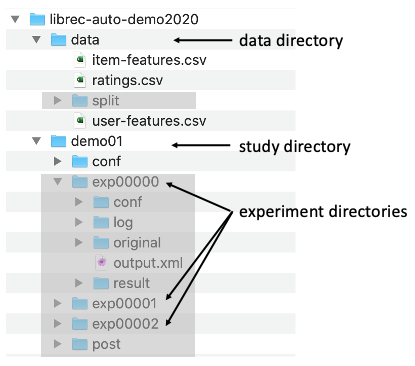
\includegraphics[width=0.8\linewidth]{imgs/la/study-dir-labeled2.png}
    \caption{Directory structure for a \libauto{} study. The shaded directories are experiment outputs managed by the system.}
    \label{fig:study-dir}
    \vspace{-0.15in}
\end{figure}

Key files in the study structure include:

\begin{description}
    \item[Data files] Ratings files and files with user and item meta-data.
    \item[Configuration files] XML-based study configuration (described in detail below).
    \item[Properties files] Input to the LibRec library.
    \item[Log files] Output from the LibRec execution.
    \item[Output files] Summary files for individual experiments and the study as whole.
    \item[Post-processing outputs] These can take a variety of forms including image, CSV and others.
\end{description}

For reproducibility, it is sufficient for experimenters to distribute their data and configuration files (\texttt{conf} directory). All other aspects of a study can be reproduced by running the \libauto{} application.

\subsection{Fairness-aware recommendation}
\label{subsec:libauto_fair_tools}

With the extensive research in literature focusing on the assessment and mitigation of unfair outcome of algorithms, several toolkits for fair machine learning have recently emerged to make such methods widely accessible.

Examples of such toolkits include: AI Fairness 360 -- an open source toolkit for mitigating bias in AI application lifecycle designed by IBM \cite{bellamy2019ai}, Fairlearn -- a toolkit for assessing and improving fairness in AI designed by Microsoft \cite{bird2020fairlearn}, Aequitas -- an open-source bias audit toolkit that allows auditing machine learning models for discrimination and bias \cite{saleiro2018aequitas}, LinkedIn Fairness Toolkit (LiFT) \cite{SriramLifT2020}, and FairSight: Visual Analytics for Fairness in Decision Making \cite{ahn2019fairsight}, just to name a few.


However these toolkits have been proposed to address issues of unfairness in classification, and the metrics and approaches they encode are not always applicable to recommender systems research. What distinguishes \libauto{}'s fairness extensions from other toolkits is its focus on evaluating and mitigating unfairness in recommender system algorithms in particular.

Although \libauto{} has been under development since 2018, the latest release incorporates several key advances that specifically support common tasks in the study of recommendation fairness. These specific fairness-aware capability of \libauto{} are (1) evaluation metrics that report on fairness aspects of recommendation output, (2) support for working with user (demographic) and item (content) features in algorithms and metrics, and (3) an optional re-ranking step in the experiment pipeline, to support what is one of the most common category of fairness enhancing techniques.
With these features, \libauto{} can support a wide range of research activities in fairness-aware recommendation, and we will be adding additional capabilities in future releases.


\subsubsection{Fairness metrics}
\label{subsubsec:libauto_fairmetrics}

In \libauto{}, we have concentrated on fairness-aware metrics that measure group fairness. However, some individual fairness metrics are also included. We intend to extend the coverage of both types of metrics in future releases. To learn more about the differences please refer to Chapter \ref{fairness} for a detailed discussion. Additionally, we have implemented these metrics from the perspective of both the providers and the consumers (the main stakeholders) in \libauto{}.

% \todo[inline]{the following paragraph is discussed in fairness chapter?}
% In addition to the group vs individual fairness distinction, recommender system fairness is also distinguished by the fact that fairness concerns may be formulated relative to multiple different stakeholders \cite{burke2017multisided,abdollahpouri2020multistakeholder}. In particular, we may be concerned about fairness towards consumers of recommendations (end-users) and providers of items being recommended. Consumer-side group fairness asks whether the system is fair to different groups of users: for example, male, female and non-binary job seekers getting recommendations of job listings. Provider-side group fairness asks whether the system is fair to different groups of item providers: for example, male, female and non-binary musical artists whose tracks are being recommended.

% We have included metrics for both types of stakeholders in \libauto{}.

% The WEA assumption is concerned with equitable treatment of users in protected groups. The WAE assumption requires that recommender systems provide individuals of a protected group (regardless of stakeholder position) to experience a similar quality of service as those in the unprotected group, according to some objective or metric deemed important to that group \cite{ekstrand2018all,ekstrand2021exploring,steck2018calibrated,yao2017beyond}.

For consumers, the common approach to measure the quality of recommendations is using accuracy-based metrics. These values are computed and compared across groups. As an example, \cite{yao2017beyond} measures and compares different types of errors among user groups. \cite{burke2018balanced} also compared the statistical parity of the precision of recommendations for different demographic groups. 

% A WSIWYG assumption asserts that all users should get similar quality of service and does not make use of a protected / unprotected group assumption. 

% \cite{steck2018calibrated} uses a diversity-based metric (KL-divergence) to measure the discrepancy between the distribution of item categories in user profile and that of her recommendations. A system that scores well on this calibration measure is considered fair in that it is providing recommendations well matched to the tastes of individual recommendation consumers, even when those tastes vary widely from the average user.
We also provide appropriate fairness metrics for providers. The first category of metrics concentrate on the results associated with protected vs unprotected provider groups. A simple way to compare these results is to look at \textit{exposure}, the likelihood that particular providers will have their items displayed in the recommendation lists of consumers \cite{liu2019farpfar,sonboli2020opportunistic}. However, displaying a recommendation to an uninterested user might not be of much value, so a utility-based (or \textit{hit-based}) alternative considers both how often items are displayed and the quality of match between the user and the item and compares these utilities between protected and unprotected providers \cite{singh2018fairness,biega2018equity}. An example of individual fairness metrics for providers is the Gini index metric, where a high (unfair) value indicates that recommendation results are highly concentrated among a few providers.

% Similarly for providers, we provide metrics appropriate under either of the WAE or WYSIWYG assumptions. Under the first assumption, we concentrate on the results associated with protected vs unprotected provider groups. A simple way to compare these results is to look at \textit{exposure}, the likelihood that particular providers will have their items displayed in the recommendation lists of consumers \cite{liu2019farpfar,sonboli2020opportunistic}. However, displaying a recommendation to an uninterested user might not be of much value, so a utility-based (or \textit{hit-based}) alternative considers both how often items are displayed and the quality of match between the user and the item and compares these utilities between protected and unprotected providers \cite{singh2018fairness,biega2018equity}. An example of individual fairness metrics for providers is the Gini index metric, where a high (unfair) value indicates that recommendation results are highly concentrated among a few providers.

\begin{table}[tb]
\centering
\caption{Fairness metrics in \libauto.}
\label{tab:fair_metrics}
\begin{threeparttable}
\begin{tabular}{lll}
\toprule
Metric            & Stakeholder Focus     & Fairness Type \\\midrule
Calibration        & consumer             & individual \\
DPF                & consumer             & group \\
Error-based        & consumer             & group \\
Gini Index         & provider             & individual \\
PPR                & consumer \& provider & group \\
Statistical Parity & provider             & group \\
\bottomrule
%\multirow{2}{*}{Diversity-based} & ILD                & provider             \\ \bottomrule
                                 
\end{tabular}
\end{threeparttable}
\end{table}


% As this discussion suggests, fairness metrics for recommender systems form a fairly complex space with many different proposals \cite{tsintzou2018bias,steck2018calibrated,beutel2019fairness,yao2017beyond,biega2018equity,castillo2019fairness,kuhlman2019fare,yang2017measuring}. 


We implement the following metrics in \libauto{} and where possible, include both consumer-side and provider-side versions of the metric, as listed in Table \ref{tab:fair_metrics}. All metrics listed here are implemented in Java and integrated with the LibRec code base: 

\todo[inline]{should be in the fairness chapter? I should not remove the claibration and DPF! lol fix them! lol}
\begin{itemize}
    \item \textbf{Calibration} \cite{steck2018calibrated}, a distribution-based metric that uses KL-Divergence to measure the difference in item category distribution between the preferences of users and their respective recommendation lists.
    \item \textbf{Discounted Proportional Fairness} (DPF), a hit-based fairness metric similar to the metric offered in \cite{castillo2019fairness} where it measures the ranking utility (nDCG) of the protected group with respect to the other groups. 
    \item \textbf{Error-based} metrics proposed in Yao et al. \cite{yao2017beyond} including value-unfairness, absolute unfairness, underestimation unfairness, overestimation unfairness. Non-parity unfairness as defined by Kamishima et al. \cite{kamishima2011fairness} is also in this group.
    \item \textbf{Gini Index} calculated over the exposure of all the providers in all recommendation lists. 
    \item \textbf{P-Percent-Rule} (PPR) discussed in \cite{biddle2006adverse}, is a two-sided extension of statistical parity \cite{barocas2016big}. 
    \item \textbf{Statistical parity}, based on the ideas discussed in \cite{zemel2013learning,ritov2017conditional}, measuring the difference in outcomes between protected and unprotected groups relative to various recommendation outcomes. Both ranking and prediction accuracy measures are supported.
\end{itemize}

In addition to this set of fairness metrics, we provide an implementation of the \textit{Intra-List Distance (ILD)} measure \cite{ziegler2005improving}, a pairwise distance between all the item features in each user’s recommendation list. This is a user-focused measure of the diversity that a recommender system provides. 

\subsubsection{Item and user metadata}
\label{subsubsec:libauto_item_user_features}
LibRec does not directly support algorithms that use item and user metadata: content-based or demographic recommendation. The ability to make use of such data is an enhancement that was made in order to implement fairness-aware algorithms and metrics: it is clear, for example, that you need to know if a user is in a protected group to know how to apply metrics like statistical parity or value unfairness. 

Our enhancements allow the algorithms and metrics to access data stored in user and item feature files. These files have a simple sparse triple format: item id (or user id), feature name, feature value. Because it is a sparse format, rows with zero values can be omitted. If the value for a feature is binary, the feature value can also be omitted and all $ \langle item, feature \rangle$ pairs that appear in the file will have a feature value of 1.

For the specific case of group fairness algorithms and metrics, the feature file must contain a feature with a binary value that represents the protected / unprotected group distinctions. Items with a value 1 for this feature will be considered protected for the purposes of metrics or algorithms. We plan to generalize this capability in future releases.

\subsubsection{Re-ranking}
\label{subsubsec:libauto_rerank}

A re-ranking algorithm takes the ranked output of a base system (usually an information retrieval or recommender system) and performs a permutation of the ordering (and usually a truncation) before sending the list to an end user. A typical application of these techniques is to enhance output diversity or fairness when the list of top candidates returned by the base system lacks these properties.

Re-rankers strive to achieve a reasonable balance between accuracy and other output properties, like fairness or diversity, by offering a tunable tradeoff between boosting protected or diverse items and including items ranked highly by the base system. 

\todo[inline]{mention in which chapter you are talking about them}
\libauto{} includes implementations of the following re-ranking algorithms:
\begin{itemize}
    \item \textbf{FAR}, defined in \cite{liu2019farpfar} and in Chapter \ref{fairness_postproc}, combines a personalization-induced and fairness-induced scores with hyper-parameter $\lambda$;
    \item \textbf{PFAR}, from \cite{liu2019farpfar} which is explainedin Chapter \ref{fairness_postproc}, adds a personalized weight to FAR, calculated based on item-features in user profile, representing the tolerance of the user for diverse results
    \item \textbf{OFAiR} is based on PFAR and allows fine-grained control of protected group promotion when there are multiple protected groups \cite{sonboli2020opportunistic}. For more details refer to Chapter \ref{fairness_postproc}
    
    \item \textbf{FA*IR} \cite{zehlike2017fa} builds a queues of protected and unprotected items and draws from each queue to build the final re-ranked list.
    \item \textbf{MMR} diversifies result lists by greedily adding items with maximal marginal relevance \cite{carbonell1998use}.
    \item \textbf{XQuAD} defined in \cite{santos2010explicit} has similar goal to MMR algorithm, but it enhances diversity with respect to specific aspects.
    \item \textbf{Calibrated Recommendations}, an algorithm closely tied to the Calibration metric above, which re-ranks recommendations to ensure a close match to the user's distribution of interests in item features~\cite{steck2018calibrated}.
\end{itemize}

The re-ranking methods are part of \libauto{} and are implemented in Python. A re-ranking script loads the original set of (large) recommendation lists computed for each user and then computes new re-ranked sub-lists for output. As noted above, re-rankers can participate in the optimization process. However, it would be inefficient to compute LibRec results multiple times if the only parameters changing were within the re-ranker. \libauto{} detects this situation and only computes results once for a given set of algorithm parameters. 


\subsection{Optimization}
\label{subsec:libauto_opt}
% \begin{markdown}

As noted above, \libauto{} supports grid search, an exhaustive method of checking each combination of values specified in order to find the optimal value. The number of experiments is determined by a cross-product of the variables. The syntax to run grid-search involves specifying specific values for a given metric. For example,

{\small
\begin{verbatim}
    <item-reg><value>0.01</value>
          <value>0.05</value></item-reg> 
\end{verbatim}
}

While grid search is guaranteed to find the optimal result within the specified parameter-value combinations, it can be expensive and time-consuming to run, particularly with a large number of variables, and depends heavily on experimenter expertise in choosing specific parameter values to sample. To overcome these difficulties, we have introduced Bayesian black-box optimization (using \texttt{optuna}), which aims to reduce the time to find an optimal combination of values \cite{akiba2019optuna}. The \texttt{optuna} package includes a number of optimization methods including the Tree Of Parzen Estimators (TPE) method, which makes probabilistically sampled estimates of optimal parameter values based on prior experimental results. In our experiments, this method outperformed other options that we considered. 

In order to use this system, an \texttt{optimize} element must be added to the configuration file (see below), and instead of the \texttt{value} syntax used to indicate possible values for grid search, the experimenter includes \texttt{lower} and \texttt{upper} elements indicating the legal range for each variable. If the metric being used is a LibRec metric then the direction of optimization is automatically determined. For user-defined metrics, the experimenter must specify the direction of optimization.

\section{Study Configuration}
\label{sec:libauto_study_config}

\libauto{} uses an XML configuration file to specify all aspects of the experimental pipeline. As noted above, a configuration file defines a \textit{study}, which computes evaluation results for a single algorithm and a single data set, possibly over multiple choices of hyperparameters, each combination of which constitutes an \textit{experiment}. The configuration file is divided into sections, some of which are optional. We devote some attention here to this file because a study of its components gives a good overview of the capabilities and flexibility of \libauto{}. A sample configuration file is shown in Figure~\ref{fig:config}.
\todo[inline]{go to the 2021 demo examples and change the config file based on that}

XML was chosen because configuration files need to be managed both by human experimenters and by the system itself. The unstructured key-value properties format used by LibRec was found to be difficult for experimenters to manage as it does not impose a natural structure on the different aspects of the configuration and makes it difficult to re-use and adapt configurations. JSON was also considered, but XML is more self-describing, which is important when the configuration must provide documentation for what experiments were performed. XML enables configuration files to be easily modularized, so that, for example, multiple studies can share the same methodology elements, preventing inadvertent misconfiguration. XML also provides facilities for validating configuration files against an XML schema, which in future versions will allow us to provide error checking of configuration files before processing them.

\begin{figure}[!htb]
    \centering
    \small{
\begin{verbatim}



<librec-auto>
    <random-seed>202001</random-seed>
    <thread-count>1</thread-count>
    <library src="system">default-algorithms.xml</library>
	
	<!-- DATA SECTION -->
	<data>
        <data-dir>../data</data-dir>
        <format>UIR</format>
        <data-file format="text">ratings.csv</data-file>
	</data>
	
	<!-- FEATURES SECTION -->
	<features>
		<appender-class>net.librec.data.convertor.appender.ItemFeatureAppender</appender-class>
		<item-feature-file>item-features.csv</item-feature-file>
		<protected-feature name="fea:new" type="item">new</protected-feature>
		<user-feature-file>user-features.csv</user-feature-file>
		<protected-feature name="fea:female" type="user">F</protected-feature>
	</features>
	
	<!-- SPLITTER SECTION -->
	<splitter>
        <model count="3">kcv</model>
        <save>true</save>
	</splitter>
	
	<!-- ALGORITHM SECTION -->
	<alg ref="alg:biasedmf">
        <similarity type="item">pcc</similarity>
        <iterator-max>25</iterator-max>
        <item-reg>
            <value>0.01</value>
            <value>0.05</value>
        </item-reg>
        <user-reg>
            <lower>0.000</lower>
            <upper>0.1</upper>
        </user-reg>
        <num-factors>20</num-factors>
	</alg>


    <!-- RERANK SECTION -->
	<rerank>
		<script lang="python3" src="system">
			<script-name>far_rerank.py</script-name>
			<param name="max_len">10</param>
			<param name="lambda">
			    <value>0.0</value>
			    <value>0.3</value>
			</param>
			<param name="binary">False</param>
			<param ref="fea:new"/>
		</script>
	</rerank>
    
    
    <!-- METRICS SECTION -->
	<metric>
        <ranking>true</ranking>
        <list-size>10</list-size>
        <class>ndcg,precision,psp</class>
        <script lang="python3" src="system">
            <script-name>ndcg_metric.py</script-name>
            <param name="list_size">10</param>
        </script>
        <protected-feature ref="fea:new"/>
	</metric>

    <!-- POST-PROCESSING SECTION -->	
	<post>
        <script lang="python3" src="system">
            <script-name>result_graphics.py</script-name>
            <param name="browser">true</param>
        </script> 
	</post>
</librec-auto>


\end{verbatim}
}

    \caption{Sample configuration file}
    \label{fig:config}
    \vspace{-0.5in}
\end{figure}

\subsection{Global elements (all optional)}
\label{subsec:lib_auto_global_elements}
The global elements establish conditions under which all aspects of the configuration file interpretation and study execution will take place.

\begin{description}
\item[random-seed]: An integer that will be used as the seed for any randomized actions that the platform takes. This ensures repeatability for experiments.
\item[thread-count]: If this is greater than zero, \libauto{} will spawn multiple threads for various tasks, including parallel execution of experiments.
\item[library]: There can be multiple \texttt{library} elements, from which algorithms, metrics and other elements can be imported. There is a default system library for algorithms (referenced in the example). An element from the library can be imported using the \texttt{ref} attribute.
\end{description}

In the example file in Figure~\ref{fig:config}, \texttt{<alg ref="alg:biasedmf"/>}` refers to the \texttt{biasedmf} (Biased Matrix Factorization) algorithm as implemented in LibRec with the default hyperparameters given in the library. The library file is also a useful reference for experimenters to see what hyperparameters a given algorithm accepts. These can be overridden by local declarations in the configuration file.

\subsection{Data Section}
\label{subsec:libauto_data_sec}

The data section indicates where the data for the study can be found. The data can be in any convenient place. However, \libauto{} will need to be able to write to this directory since it will by default add new data split directories here. \footnote{Note that, for LibRec compatibility, there are two different places where the label ``format'' is used. The \texttt{format} element indicates the columns in the ratings file. The \texttt{format} attribute of the \texttt{data-file} element is the file format of the ratings file: LibRec supports text and AIFF file formats.}

\subsection{Feature Section (optional)}
\label{subsec:libauto_feature_selection}

LibRec is heavily focused on collaborative algorithms, so the basic form for input data is the user/rating matrix. However, as noted above, for content-oriented algorithms and for fairness-aware algorithms and metrics, it may be necessary to have item metadata and/or user demographic data. The \texttt{feature} element allows experimenters to include either item or user features as input to a study's algorithm or metrics. 

\subsection{Splitter Section}
\label{subsec:libauto_splitter}
A variety of different evaluation strategies are employed by recommender systems researchers to evaluate algorithms. K-fold cross-validation is a common one, and LibRec supports multiple variants on this approach. 

The example in Figure~\ref{fig:config} directs \libauto{} to perform five-fold cross-validation using 80\% of each user's data for training and 20\% for testing in each fold. The splits will be saved to the data directory, and can be re-used in subsequent experimentation. 

The configuration file also supports fixed training and test files supplied by the experimenter and temporal splitting (when dates are available for ratings). 

\subsection{Algorithm Section}
\label{subsec:libauto_algos}
LibRec supports more than 70 recommendation algorithms, each linked to a paper from the scientific literature that it implements. A default algorithms library contains a number of the most common algorithms and complete lists of their hyperparameters with default values.

Typically, a study will consist of multiple experiments over different algorithm hyperparameters. As noted in Section~\ref{subsec:libauto_opt}, \libauto{} supports both grid search and Bayesian black-box optimization. In Figure~\ref{fig:config}, the weight for the item regularization term (\texttt{item-reg}) is being varied across two values, 0.01 and 0.05. This information tells the system to conduct two experiments using the given weight values. Any number of hyperparameters can be searched over. The system will conduct an experiment for every combination of values (Cartesian product), so the number of experiments can be quite large.

\subsection{Optimize Section (optional)}
\label{subsec:libauto_opt}
The black-box optimization capability requires the use of a separate \texttt{optimize} element to specify what metric is used for optimization and how many iterations are to be performed. For example,

{\small
\begin{verbatim}
<optimize><metric>precision</metric>
          <iterations>25</iterations></optimize>
\end{verbatim}}

This option cannot be combined with grid search. If it is used, instead of providing a list of values associated with a parameter (the \texttt{value} element), we provide an upper and lower bound to the search range.

{\small
\begin{verbatim}
<item-reg><lower>0.01</lower>
          <upper>0.05</upper></item-reg>
\end{verbatim}}

\subsection{Metrics Section}
\label{subsec:libauto_metrics}

A study can employ multiple metrics. LibRec supports over 20 different metrics for evaluating recommender system performance. There are two basic types: \textit{error metrics}, which compare the predictions produced by an algorithm with known ratings from the test set, (for example, RMSE), and \textit{ranking metrics}, which evaluate a ranked list of results produced for each user in the training data (for example, Precision@10). Although multiple metrics can be used, only one type of metric can be used at a time since these methodologies are quite different in how they make use of the training data. Ranking metrics (like Precision@10 shown in the example) require the \texttt{ranking} element to be true and a list-size to be specified.

Fairness-aware metrics require a \texttt{protected-feature} element. The current release requires this to be a binary feature drawn from the item or user feature file. Items (or users) associated feature value of 1 will be considered protected for the purposes of a fairness metric. This value is also used by fairness-aware algorithms in LibRec.

\libauto{} supports custom metrics defined as Python scripts, similar to re-ranking scripts described below. Implementers can make use of generic error or ranking metric abstract classes for building their metrics, minimizing the amount of implementation effort. This eliminates the need to program such metrics in Java and re-compile the LibRec executable.

If black-box optimization is used, the optimizer needs to know which direction of a metric is considered ``good'': note that large RMSE is bad, but large nDCG is good. This property is pre-defined for built-in metrics, but for custom metrics, a flag must be included in the metric \texttt{script} declaration to indicate whether to optimize for larger or small values of the metric.  

\subsection{Rerank Section (optional)}
\label{subsec:re-ra}
For a study that includes re-ranking, the re-ranking script is specified in a \texttt{rerank} element. Note that all re-ranking is done by script resources and these can be easily customized by experimenters. Currently, only Python scripts are supported.

The configuration for a re-ranker indicates the parameters to be passed. In the following example, we see that the \texttt{far-rerank.py} script is being used, which implements the re-ranker described in \cite{liu2019farpfar} and Section \ref{sec:farpfar}. The \texttt{max\_len} parameter tells the script how many items will be returned for each user from the re-ranked set. Other parameters are algorithm-specific controls on the re-ranking process. The FAR algorithm defined in \cite{liu2019farpfar} uses the \texttt{lambda} and \texttt{binary} parameters shown here.

{\small
\begin{verbatim}
<rerank>
   <script lang="python3" src="system">
      <script-name>far-rerank.py</script-name>
         <param name="max_len">10</param>
         <param name="lambda">
            <value>0.3</value>
            <value>0.0</value>
         </param>
         <param name="binary">False</param>
   </script>
</rerank>
\end{verbatim}}

Note that a re-ranking step can participate in the optimization aspects of \libauto{}. In the example above, we explore two different values of \texttt{lambda} in combination with whatever other hyperparameters are being searched. (Black-box optimization is not yet available for re-ranker parameters, but is a planned feature.)

\subsection{Post-Processing Section (optional)}
\libauto{} supports the post-processing of study results. There are existing scripts for producing simple visualizations (see Figure~\ref{fig:viz}), for producing CSV files for further analysis, and for posting experimental results to Slack and Dropbox (see Figure~\ref{fig:slack}). The latter are useful for experiments with longer run-times. There is a script provided for encrypting application API keys so that they do not need to be shared (insecurely) in the configuration file. 

\todo[inline]{drop this}
\begin{figure}[!htb]
    \centering
    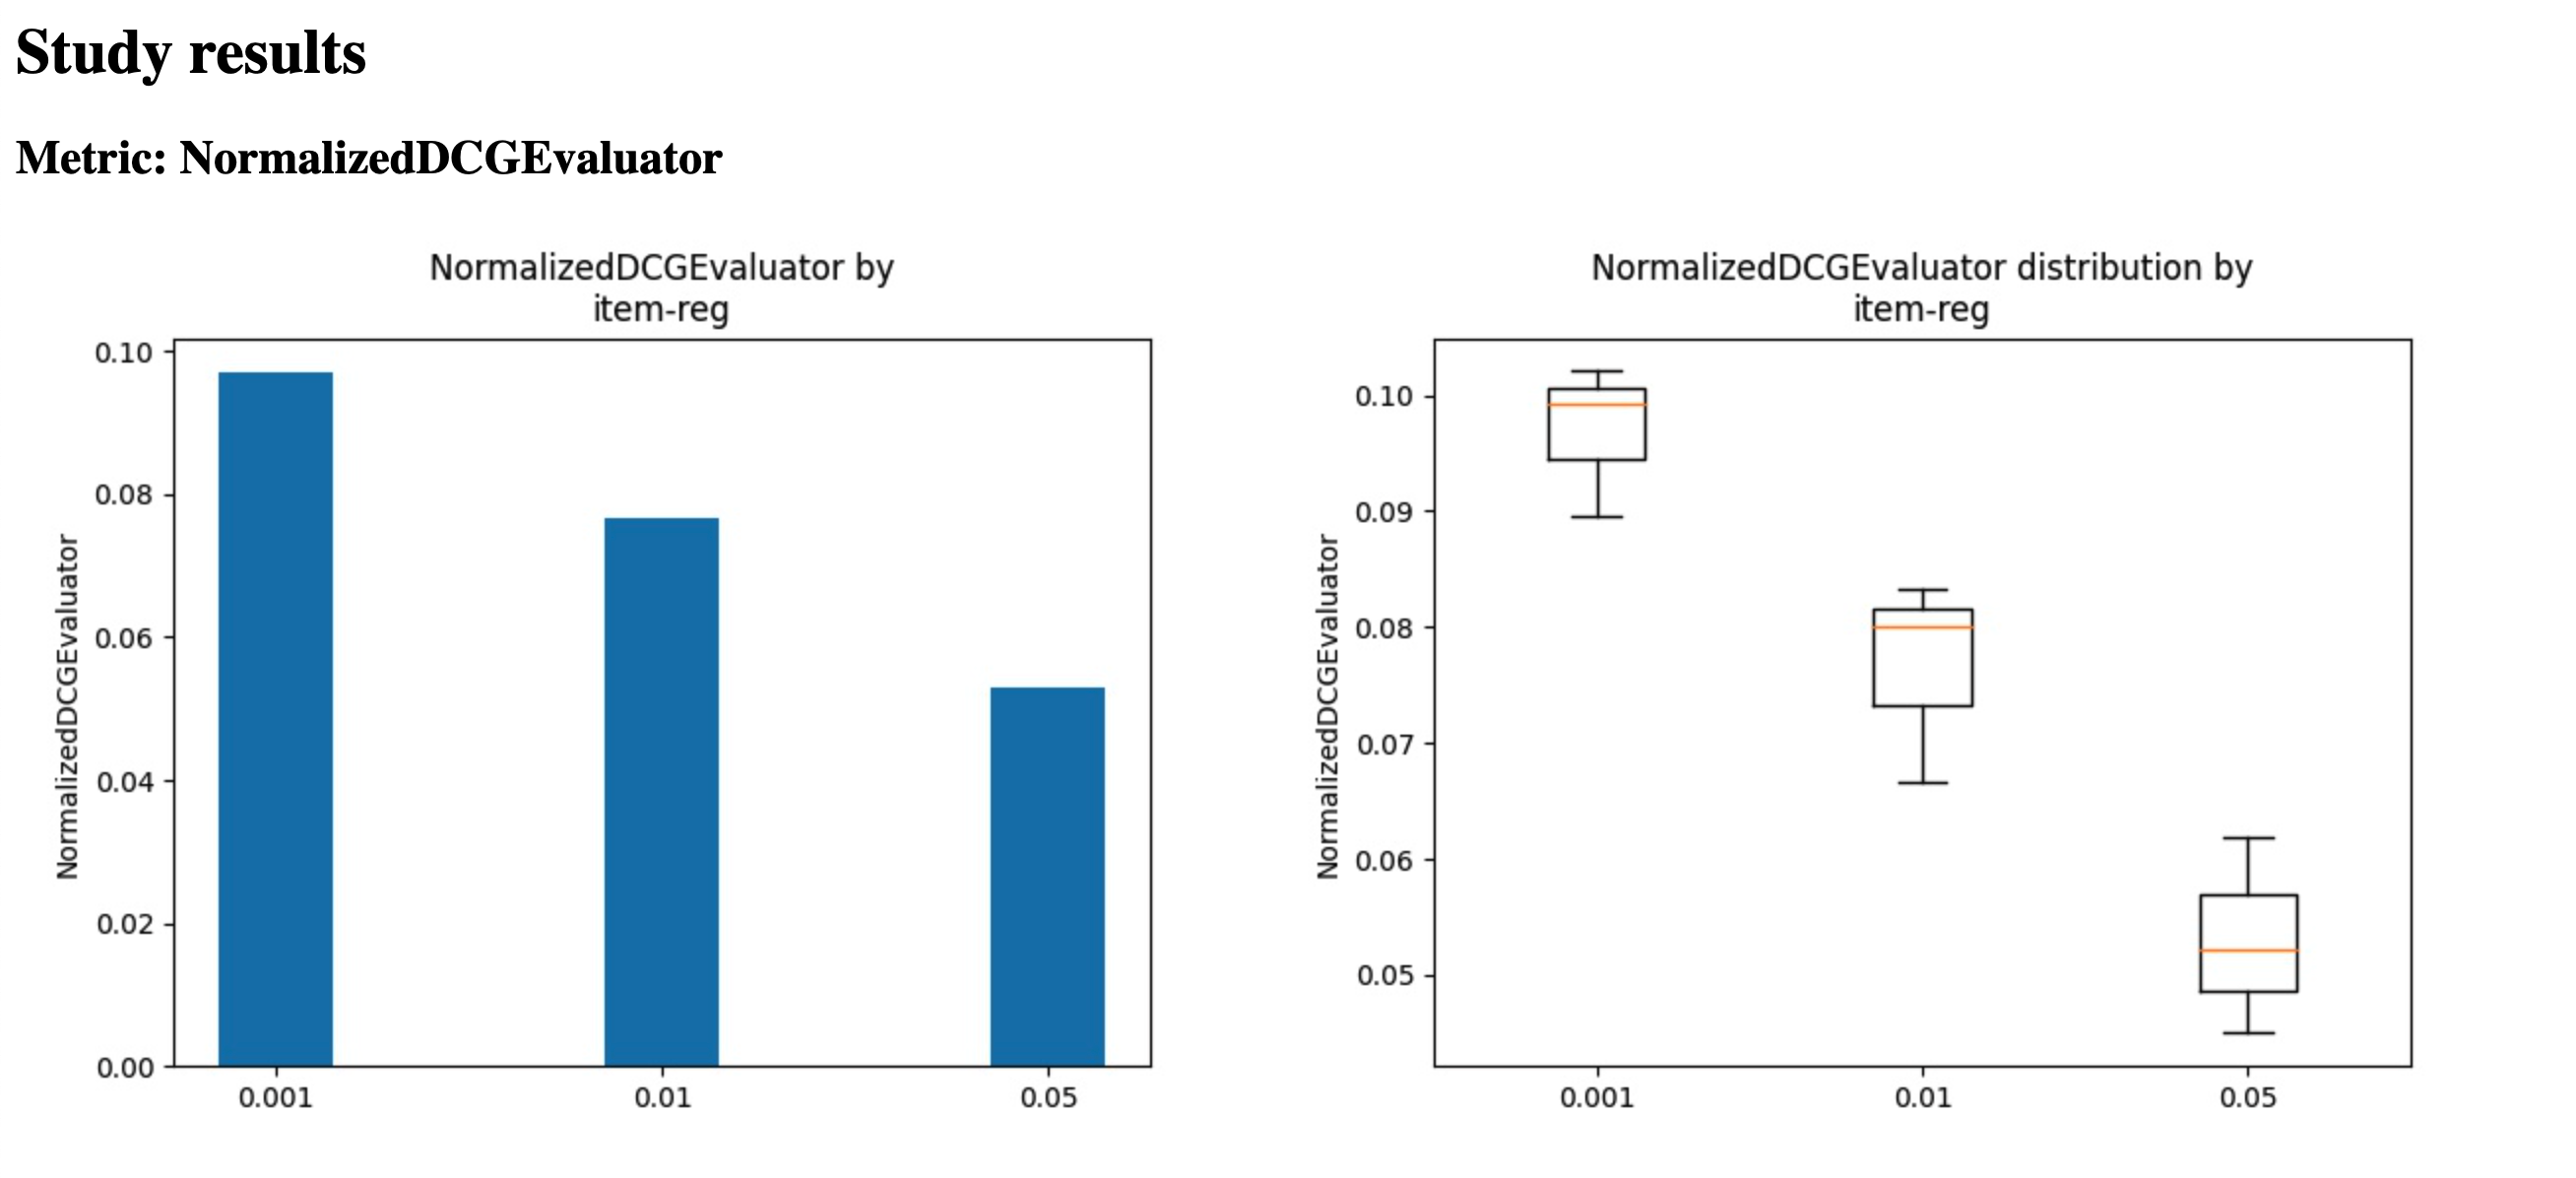
\includegraphics[width=0.8\linewidth]{imgs/la/sample-output.png}
    \caption{Sample auto-generated study output visualizations. These simple plots support experimenters in providing a quick analysis of study outcomes.}
    \label{fig:viz}
    \vspace{-0.15in}
\end{figure}

\begin{figure}[!htb]
    \centering
    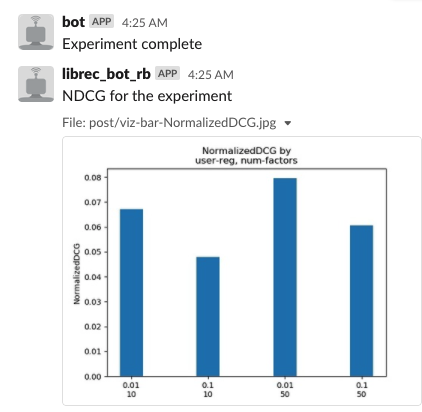
\includegraphics[width=0.6\linewidth]{imgs/la/slack-post.png}
    \caption{Sample auto-generated Slack posts. Such notifications provide experimenters and research teams with asynchronous notifications of study progress.}
    \label{fig:slack}
    \vspace{-0.15in}
\end{figure}

\section{Related Work}

With the rapid growth of published recommendation algorithms, the concern about reproducibility of models in the research community has given rise to the need of having standard implementations for models and evaluation metrics. Many of the recommendation algorithms lack public implementations or those that have one, are inconsistent in details. \libauto{} is a response to this need, but it should be noted that there many other recommender systems libraries have been created and offered to the research community, beginning with earlier systems such as MyMediaLite \cite{MyMediaLite} and continuing through newer releases such as Microsoft Recommenders \cite{MicrosoftRecommenders} and RecBole \cite{recbole}. However, none of these libraries offer the precise combination of features that are found in \libauto{} and some are no longer being maintained.

There are multiple differences between the existing recommender systems libraries from the coverage of newer algorithms in the library to incorporation of fairness-aware metrics and algorithms.

One of the key aspects of \libauto{} is its incorporation of fairness-aware metrics and algorithms. As noted above, the platform has strong support for re-ranking, perhaps the most common fairness-aware recommendation technique, and it includes examples of re-ranking algorithms from the research literature, as described in Section \ref{subsubsec:libauto_rerank}. Also, \libauto{} supports metrics for both consumer- and provider-side fairness as noted in Section \ref{subsec:libauto_metrics}. No other existing library has these capacities. 

Another important difference between \libauto{} and existing libraries is its large collection of algorithms (~70) drawn from LibRec itself. Many existing libraries, for example, RecommenderLab \cite{hahsler2015recommenderlab}, LKPY \cite{LensKit2020}, and Surprise \cite{Hug2020} concentrate on a relatively small handful of algorithms.

Microsoft Recommenders \cite{MicrosoftRecommenders} includes 31 recommendation algorithms (including the most current work in deep learning and neural networks) and RecBole \cite{recbole} includes 72 recommendation models from the recent years (mostly 2017-2020), but these libraries have almost no overlap with those included in LibRec and so can be thought of as useful complements. We have integrated some of the algorithms from the Microsoft library in particular as part of our next major release, as described below.


Finally, \libauto{} stands apart for its use of explicit algorithm configuration and support for unattended operation. While Jupyter notebooks are very convenient for interactive exploration of algorithm properties, we have found that large-scale experimentation (especially for researchers on limited compute budgets) is best supported through the ability to configure and run batch processes and this has been considered a primary use case since the project's inception.

% \todo{filling the following table}
% \todo{Should I have the same thing for fairness related libraries?}

% \begin{table}[!htb]
% \centering
% \caption{recommender system libraries}
% \label{tab:fair_libs}
% % \resizebox{\textwidth}{!}{
% \rotatebox{90}{
% \begin{tabular}{lllllll}
% \toprule
% Library name        & Language      & number of algorithms (metrics)      & optimization       & Environments    & maintained      & License\\\midrule
% Librec-auto         & Python           &  \\
% Librec              & Java             &  \\
% Librec TRSL &
% Recbole        &              &  \\
% MicrosoftRecommenders         &              &  \\
% LensKit Python (LKPY)            &  \\
% MyMediaLite                &  &  \\
% % MyMediaLite 3.11 [6] is an open-source C# platform5
% % for recommender systems
% % experimentation6
% % . It supports both ranking and rating prediction tasks and provides a wide range of recommendation algorithms for running experiments. It
% % also has useful functionalities like grid search for optimizing hyperparameters
% % and model saving .
% % Even though MyMediaLite saves computed models, it does not save the intermediate files and outputs. Also, it does not have a configuration file for specifying
% % the hyperparameters for its recommendation algorithms.

% Apache Mahout             &  \\
% EasyRec             &  \\
% Apache Mahout             &  \\
% RecommenderLab             &  \\
% DRecPy              &   \\
% Elliot              & \\
% DUINE recommender   & \\
% DeepRec     &\\


% \bottomrule
% %\multirow{2}{*}{Diversity-based} & ILD                & provider             \\ \bottomrule
                                 
% \end{tabular}
% }
% \end{table}
% \todo[inline]{Maybe include number of metrics. Add TRSL fork of LibRec as an entry.}


\section{Discussion and Future Directions}
The \libauto{} project is driven by the needs of recommender systems experimentation and education and continues to evolve. Its key features (explicit configuration, built-in parameter optimization, computationally-efficient result handling) were all requirements that surfaced within our research work. Newer capabilities in the area of fairness-aware recommendation and re-ranking have a similar genesis and proven practical value. 

We note that \libauto{} does not directly support all popular methodologies for recommender systems evaluation. In particular, it supports only batch evaluation, and not iterative and dynamic evaluation as required by bandit and reinforcement learning paradigms. There are other platforms, for example RecoGym \cite{rohde2018recogym} and RecSim NG \cite{mladenov2021recsim}, that support this type of methodology and we do not anticipate the need to evolve our system in this direction. 

\subsection{Algorithm integration}
One of the key requirements for future releases is that the platform makes it easy to experiment with algorithms other than those implemented in LibRec. By the time of publication, we expect to have released interfaces to a popular recommendation library: Microsoft's Recommenders library~\cite{argyriou2020microsoft}. 

% LibFM~\cite{rendle2012factorization}
% LibFM\cite{rendle2012factorization} is a factorization machine (FM) software tool written in C++, that features stochastic gradient descent (SGD) and alternating least-squares (ALS) optimization, as well as Bayesian inference using Markov Chain Monto Carlo (MCMC) for regression and classification tasks. It also contains methods for optimizing an FM model with respect to ranking. 

As noted above, Microsoft Recommenders \cite{MicrosoftRecommenders} is an open-source platform for recommender systems development and evaluation. This Python-based tool includes 31 recommendation algorithms including some recent deep learning algorithms, for example, Neural Recommendation with Multi-Head Self-Attention (NRMS) \cite{wu2019neural}. While the platform includes many capabilities for data handling and evaluation, these are handled by \libauto{} in our integration. We draw only from the algorithm implementations. 

An experimenter accesses non-LibRec platforms through custom wrapper scripts to which parameters are passed. For example, the algorithm configuration element below invokes the xDeepFM \todo{can't read robin's comment} algorithm using the \texttt{msrec-wrapper.py} and passing arguments needed by this algorithm.

{\small
\begin{verbatim}
<alg>
   <script lang="python3" src="system">
      <script-name>msrec-wrapper.py</script-name>
         <param name="model">xdeepfm</param>
         <param name="epochs">200</param>
         <param name="batch_size">256</param>
         <param name="learning_rate">1e-3</param>
         <param name="cross_reg">0.0001</param>
         <param name="embed_reg">0.0001</param>
         <param name="num_factors">100</param>
         <param name="feature_count">1000</param>
         <param name="field_size">10</param>
   </script>
</alg>
\end{verbatim}}

\subsection{Fairness-aware aspects}
\libauto{} is unique in its library of recommendation re-ranking algorithms, and this aspect of the project is being actively developed. The current library of re-rankers only includes \textit{listwise} re-rankers that optimize one recommendation list at a time. There is a thread of fairness- and diversity-aware research that studies \textit{batch} re-rankers that optimize over the entire collection of recommendation lists at once: see, for example, \cite{surer2018multistakeholder,patro2020fairrec,mansoury2020fairmatch}. We plan to extend our library of re-rankers to include this class of algorithm, and, as we have with the listwise class, provide base implementations with which researchers can construct their own.

Similarly, while \libauto{} has a large variety of fairness metrics and supports both consumer-side and provider-side analysis, this capability will be enhanced in future versions. There remain some fairness definitions in the literature that we have not yet implemented, and some of our existing implementations are not as flexible as might be desired. In particular, we note that currently all fairness-aware aspects of any given study must be focused on a single side of the analysis (consumer or provider) and all group fairness aspects are controlled by the same definition of what is protected. We are extending this capability to allow (for example) re-ranking under one fairness definition and evaluating based on another. We are also planning to relax the constraint that protected groups must be defined by binary features, so that experimenters can control how protected groups are defined without having to produce new feature files in which the distinction is encoded. 


\subsection{Other enhancements}

While the system supports experimenters in planning, executing and evaluating individual studies, it does not support more general research workflows that might involve the comparison of multiple algorithms. For this higher-level support, we are working to integrate ClearML\footnote{https://clear.ml/}, an open-source machine learning management platform. A prototype of this integration is already in use.

\libauto{} also does not currently support Bayesian optimization in combination with re-ranking. We anticipate adding support for this in the near future.  

Finally, we are seeking to make \libauto{} more accessible to new users through the development of a setup wizard that automates the creation of study directories and configurations for typical use cases. The initial version of this wizard is part of the current codebase and we have plans for its continued enhancement. 

\todo{connection to the next chapter, conclusion?}

\subsection{Contributions}

\libauto{} has been presented in multiple conferences. The system was introduced through a demo at the ACM Recommender Systems conference in 2018 \cite{mansoury2018automating}, was presented at the Algorithm Selection and Meta-Learning Workshop (AMIR) at the European Conference on Information Retrieval (ECIR) in 2019 \cite{mansoury2019algorithm}. It was also presented to the audience of the ACM Conference on Fairness, Accountability and Transparency as a tutorial in 2020 \cite{burke2020facct_libauto} and presented as a demo at the ACM Recommender Systems conference in 2020 \cite{Sonboli2020FARLA}. Finally \libauto{} was presented as a resource paper at the ACM International Conference on Information and Knowledge Management (CIKM) in 2021. You can refer to the evolution timeline of \libauto{} in Figure \ref{fig:librec-auto-evolution}.

\todo[inline]{replace LIBFM with Optuna}


\begin{figure*}[!htb]
    \centering
    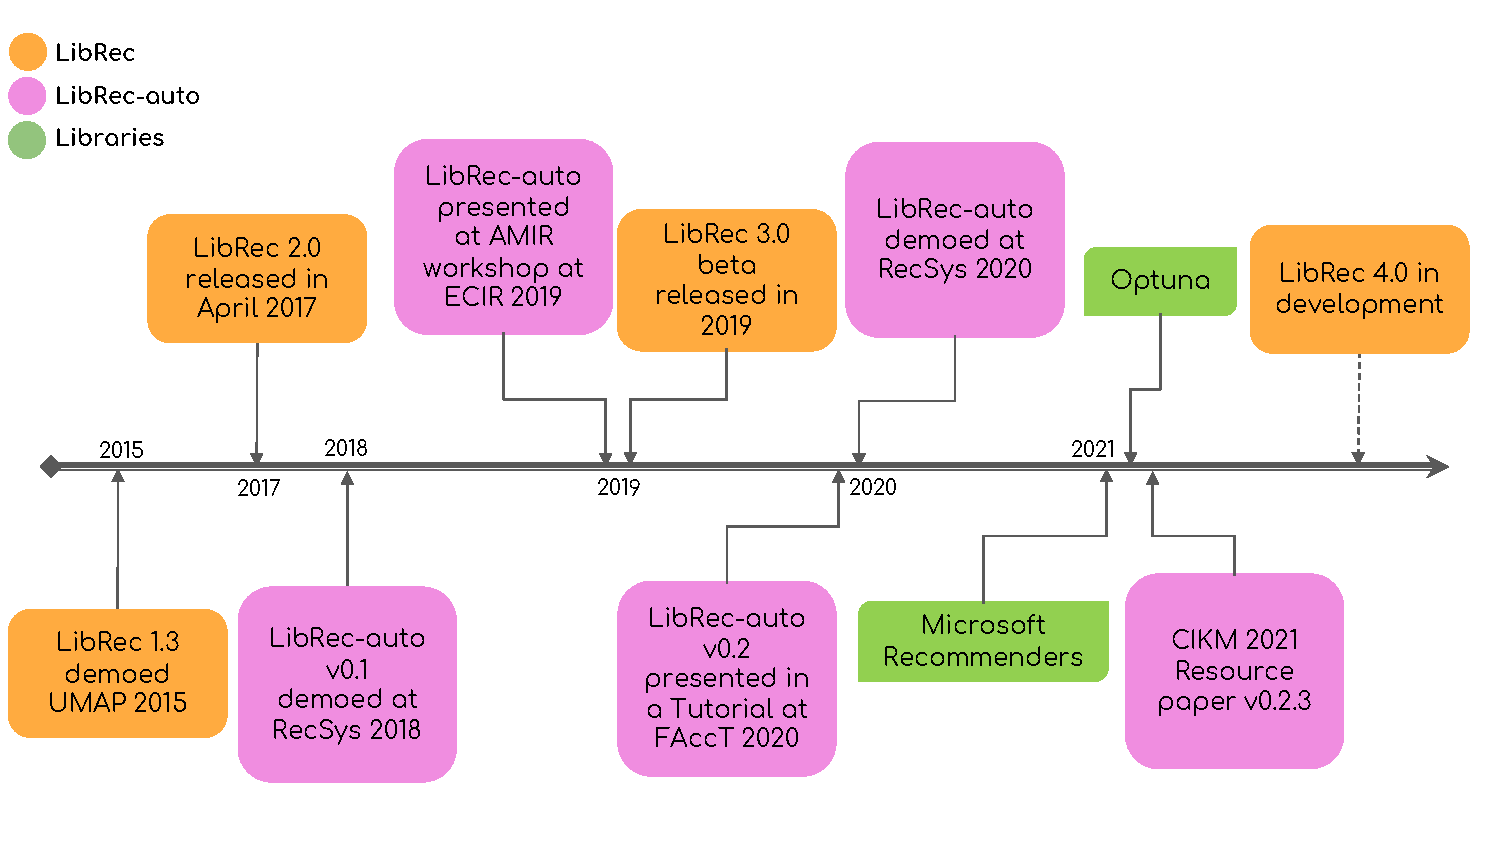
\includegraphics[width=0.95\linewidth]{imgs/la/librec-auto-evolution.pdf}
    \caption{The evolution timeline of \libauto{} (2018-2021). Every extension of \libauto{} is shown in pink and the release of LibRec itself is shown in Orange. Additional libraries that were added to the current release are shown in green}
    \label{fig:librec-auto-evolution}
    \vspace{-0.15in}
\end{figure*}

I have been working on this library throughout my PhD program and I used this tool for many experiments in this dissertation. 
This library has been evolving in 2018 and our aim is to keep evolving it in order to provide better experimental capabilities for the research community. 